\documentclass{PoS}
\newcommand{\as}{\\[14pt]}
\newcommand{\s}{\\[7pt]}
\newcommand{\is}{\\[2pt]}
\newcommand{\no}{\noindent}
\newcommand{\ka}{\hspace*{0.5cm}}
\newcommand{\ma}{\hspace*{1cm}}
\newcommand{\ga}{\hspace*{1.5cm}}
\newcommand{\li}{\left|}
\newcommand{\re}{\right|}
\newcommand{\const}{\text{const.}}
\newcommand{\z}{\text}
\newcommand{\terminal}[1]{\colorbox{black}{\textcolor{white}{{\fontfamily{phv}\selectfont \scriptsize{#1}}}}}
\newcommand{\plugin}[1]{\textit{\flq#1\frq}}
\newcommand{\ra}{$\rightarrow$ }
\definecolor{cadmiumgreen}{rgb}{0.0, 0.42, 0.24}
\newcommand{\itemfill}{\setlength{\itemsep}{\fill}}
\newcommand{\orderof}[1]{$\mathcal{O}\left(#1\right)$}
\newcommand{\fig}[2]{\begin{figure}\centering\includegraphics[height={#2}\textheight]{#1}\end{figure}}
\newcommand{\figc}[3]{\begin{figure}\centering\includegraphics[height={#2}\textheight]{#1}\caption{#3}\end{figure}}
\newcommand{\figp}[2]{\begin{figure}\centering\includegraphics[width={#2}\textheight, angle=-90]{#1}\end{figure}}
\newcommand{\figpc}[3]{\begin{figure}\centering\includegraphics[width={#2}\textheight, angle=-90]{#1}\caption{#3}\end{figure}}
\newcommand{\test}[1][bla]{#1}
\newcommand{\subfig}[4][0.45]{\begin{subfigure}{{#1}\textwidth}\centering
			\includegraphics[height={#3}\textheight]{#2}
			\caption{#4}\end{subfigure}}
\newcommand{\subfigp}[4][0.45]{\begin{subfigure}{{#1}\textwidth}\centering
			\includegraphics[width={#3}\textheight, angle=-90]{#2}
			\caption{#4}\end{subfigure}}

\usepackage[printonlyused]{acronym}
\usepackage{siunitx}
\usepackage{varioref}

\graphicspath{ {pics/} }
\makeatletter
\def\input@path{ {sections/} }
\makeatother

\title{Diamond Detector Technology: Status and Perspectives}
\ShortTitle{Diamond Detector Technology: Status and Perspectives}

\author{\speaker{Michael Reichmann}%
        \thanks{The full list of RD42 authors is provided in the appendix.}\\
       Eidgenoessische Technische Hochschule Zuerich (CH)\\
       E-mail: \email{michael.reichmann@cern.ch}}

\abstract{Here could be your abstract ;-)}

\FullConference{The European Physical Society Conference on High Energy Physics\\
         5-12 July\\
         Venice, Italy}

\makeindex
\begin{document}

%============= 1 =============
\section{Introduction}
The upgrade of the \ac{LHC} to the \ac{HL-LHC} from \SIrange{2023}{2025}{} \cite{hllhc} will push the luminosity limits even above the original design values of the \ac{LHC} and will therefore hopefully give us even more insights in the fundamental nature of the universe. In 2028 an instantaneous luminosity of \SI{5e34}{\per\centi\meter\squared\per\second} is aspired. This will be equivalent to a fluence of \SI{2e16}{n_{eq}\per \centi\meter^2} \cite{auzinger} for the innermost tracking layer at a distance of \SI{\sim30}{\milli\meter} from the interaction point. In this environment, pixel hit rates of \SI{3}{\giga\hertz\per\centi\meter^2} are expected. The current pixel detectors are designed to withstand \SI{\sim300}{\per\femto\barn} and thus the full detector would have to be replaced about every semester. This fact led to research and development of various radiation hard detector designs and materials.\\
Its large displacement energy and a high band gap of \SI{5.5}{\electronvolt} at \SI{305}{\kelvin} make diamond an excellent candidate for such a radiation tolerant detector which is why the RD42 Collaboration is investigating \ac{sc} and \ac{p} \ac{CVD} diamond as an alternative for precision tracking detectors for over two decades. In order to grow high quality detector grade diamonds, RD42 collaborates with industrial companies. All shown results are acquired with \ac{sc}\ac{CVD} diamonds produced by Element Six Technologies \cite{e6} and \ac{p}\ac{CVD} diamonds produced by II-VI Incorporated \cite{II6}. The two companies use propriety \ac{CVD} processes to fabricate their products. Both diamond types are grown on homo-epitaxial substrates with the difference that for \ac{sc}\ac{CVD} another \ac{sc}\ac{CVD} diamond is used as substrate and thus its size is limited to \SI{\sim0.25}{\centi\meter\squared}. However, for the \ac{p}\ac{CVD} a diamond powder can be used as a substrate whereby it can be grown to wafers of diameters up to \SI{6}{inch} \cite{felix}. In various studies it was found out that compared to corresponding silicon detectors, diamond is at minimum three times more radiation hard \cite{deboer}, has at least a two times faster charge collection \cite{pernegger} and its thermal conductivity is four times higher \cite{zhao}.\\
Due to the very high particle fluxes and radiation doses expected for the \ac{HL-LHC} it is very important to understand the behaviour of future detectors in this environment. The RD42 Collaboration has studied \ac{CVD} diamond detectors with irradiation doses up to \SI{2.2e16}{p\per\centi\meter^2}. In order to build even more radiation hard detectors a new technology - 3D detectors \cite{3D} - is investigated. The clever design of these detectors allows to heavily reduce the drift distance of the created charge carriers without reducing the total number of the created electron-hole pairs. Since the the signal behaviour of diamonds at high fluxes is uncertain, high rate studies are performed at \ac{PSI} with nearly \acp{MIP} and tunable particle fluxes from the order of \SI{1}{\kilo\hertz\per cm^2} up to the order of \SI{10}{\mega\hertz\per cm^2}.

%============= 2 =============
\section{Diamond Detectors at CERN}
It is essential for all modern collider experiments to have an online monitoring of the beam conditions. Since it is important to have these detectors as close as possible to the beam all of the four main experiments at the \ac{LHC} are using detectors with diamond sensors. ATLAS \cite{gorisek}, ALICE, CMS \cite{bartz} and LHCb \cite{domke} all make use of various \acp{BCM} and/or \acp{BLM} based on both \ac{CVD} type diamonds for live background estimations and luminosity measurements.\\
As an upgrade of the \ac{BCM} during the long shutdown in 2014 ATLAS installed the \ac{DBM}. Its purpose is to measure an instantaneous (bunch-by-bunch) luminosity and the bunch-by-bunch position of the beam spot. With its eight telescopes à three detector planes it adds tracking capability to the existing precise \ac{ToF} measurements of the eight pad detectors of the \ac{BCM}. The usage of state of the art pixel detectors based on the FE-I4b readout chip strongly increases the spatial resolution of the monitor and due to its projective geometry pointing towards the interaction region it also can distinguish particles coming from collisions and background \cite{dbm}. The telescopes whereof the sensors of two are made out silicon and the other six out of \ac{p}\ac{CVD} diamond are positioned symmetrically around the beam pipe on both sides of the interaction point and are shown in \vref{dbm}.
\begin{figure}
	\centering
	\begin{subfigure}{.66\textwidth}
		\centering
		\vspace*{.05\textheight}
		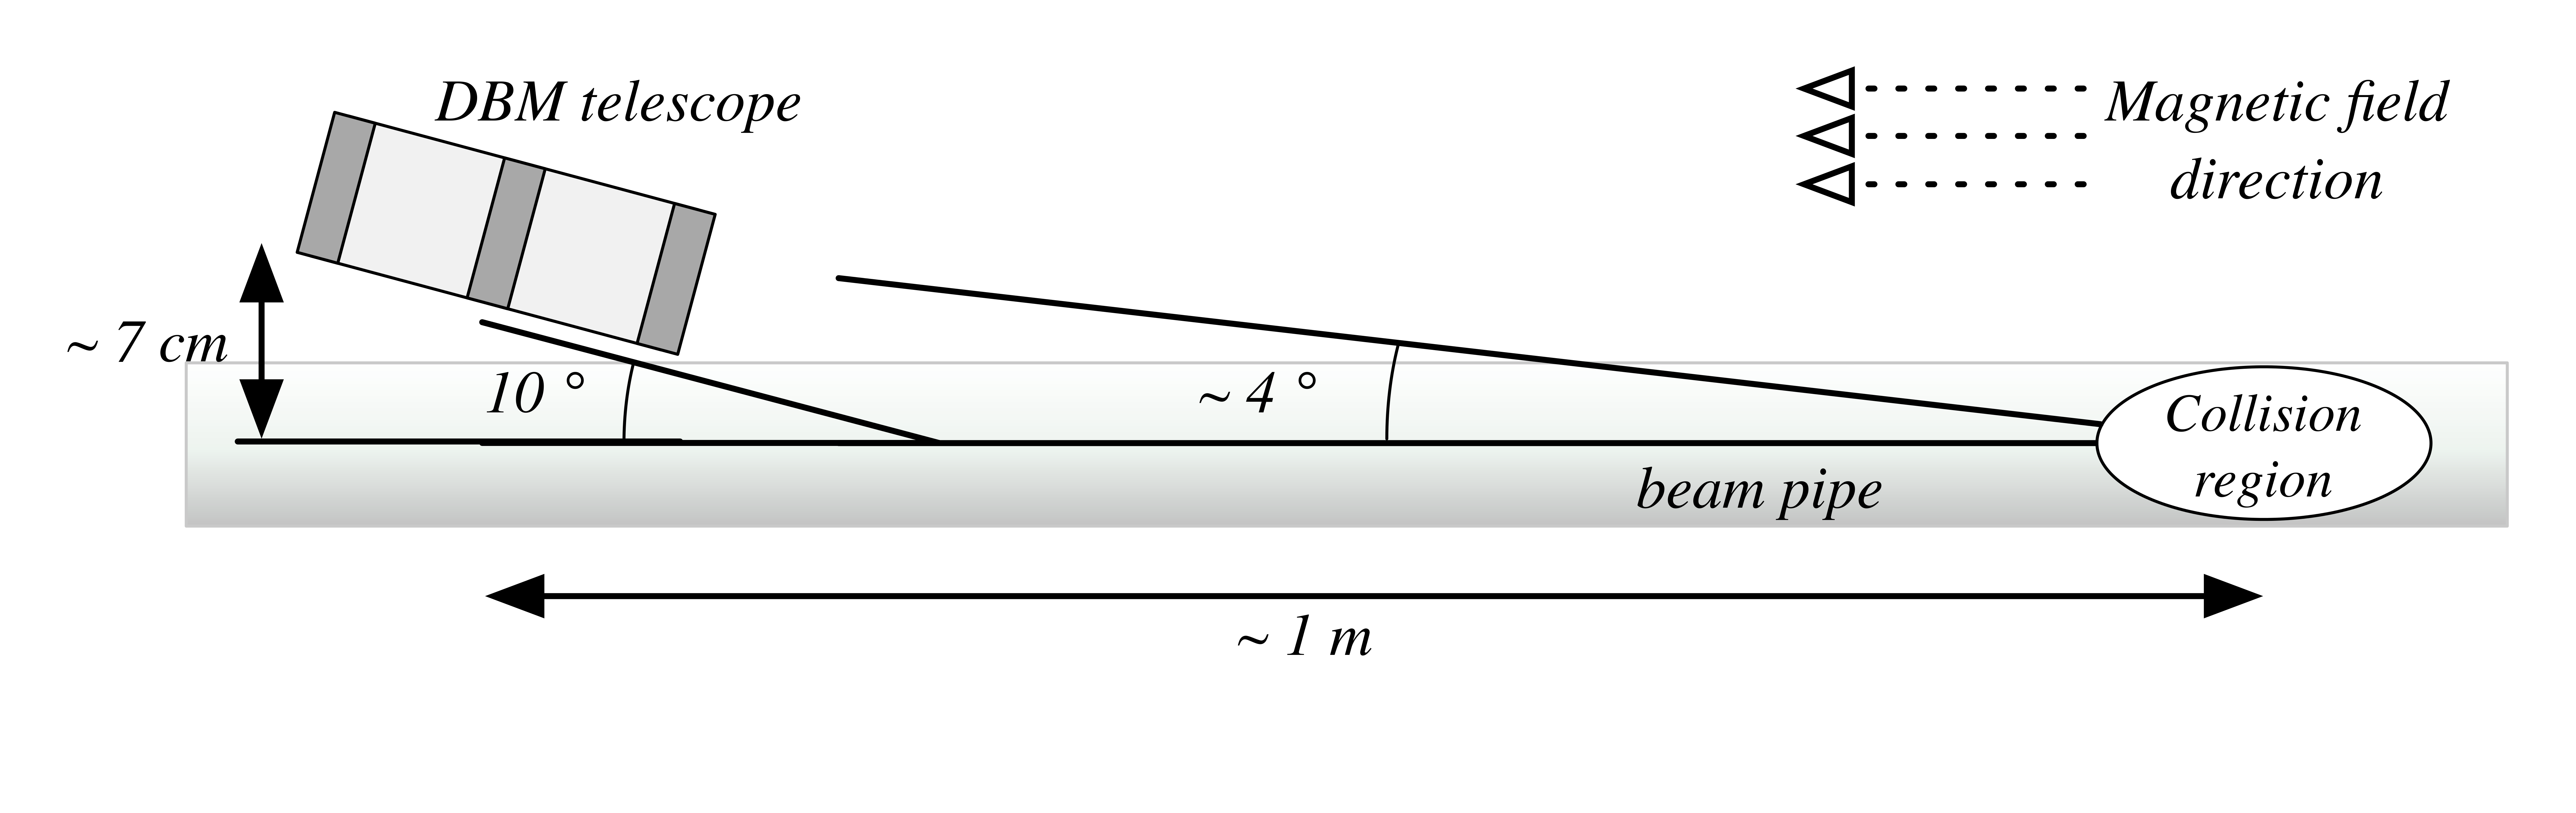
\includegraphics[height=.14\textheight]{dbm1.png}
		\vspace*{.02\textheight}
		\caption{positioning and alignment}
	\end{subfigure}
	\subfig[.33]{DBM2.png}{.23}{four mounted telescopes}
	\caption{\ac{DBM} telescope}
	\label{dbm}
\end{figure}


%============= 3 =============
\section{Radiation Tolerance}\label{rad}
In order to probe the radiation tolerance of \ac{CVD} diamond sensors several radiation studies have been performed varying the types and energies of damaging particles. The sensors were irradiated with protons of different energies (\SI{24}{\giga\electronvolt}, \SI{800}{\mega\electronvolt}, \SI{70}{\mega\electronvolt}, \SI{25}{\mega\electronvolt}), \SI{\sim1}{\mega\electronvolt} reactor neutrons and \SI{200}{\mega\electronvolt} pions up to a maximum dose of \SI{2.2e16}{p\per\centi\meter^2} which is equivalent to \SI{\sim500}{\mega rad}.\par

\begin{table}[t]
	\centering
	\footnotesize
	\begin{tabular}[c]{l|l|l}
		\noalign{\hrule height 1pt}
		\multicolumn{1}{c|}{\textbf{Particle}} & \multicolumn{1}{c|}{\textbf{Energy}} & \multicolumn{1}{c}{\textbf{Relative $\upkappa$}} \\\hline
		Proton 	& \SI{24}{\giga\electronvolt} 	& $1.0$ 			\\\hline
				& \SI{800}{\mega\electronvolt} 	& $1.79 \pm 0.13$ 	\\\hline
				& \SI{70}{\mega\electronvolt} 	& $2.4 	\pm 0.4$ 	\\\hline
				& \SI{25}{\mega\electronvolt} 	& $4.5 	\pm 0.6$ 	\\\hline
		Neutron	& \SI{\sim1}{\mega\electronvolt} 	& $4.5 	\pm 0.5$ 	\\\hline
		Pion	& \SI{200}{\mega\electronvolt} 	& $2.5 	- 3$ 		\\
		\noalign{\hrule height 1pt}
	\end{tabular}
	\caption{Damage constants for various irradiations normalised to \SI{24}{\giga\electronvolt} protons}
	\label{trad}
\end{table}	

In order to build a detector out of a \ac{CVD} diamond sensor a specific recipe is applied where the diamond is cleaned and metallised \cite{kagan}. Depending on the geometry of the metallisation pattern, pad, strip and pixel detectors can be built. For the radiation studies a strip pattern was chosen in order to correlate pulse height and position information.\par
%%%%%%%%%%%%%%%%%%%% PREPARATION %%%%%%%%%%%%%%%%%
% In a first step the surface of the raw diamond sensor has to be polished, cleaned and prepared for photo-lithography. Using the photo-lithography a metallisation pattern is then brought on the surface of the diamond. Depending on the pattern three types of detectors can be created: pad, strip and pixel detectors. This process is done for both of the sides of the diamond sensor whereby an almost edgeless design is obtained. By using a segmentation of the detector one can probe the charge of the detector depending on the position of the sensor which is critical for radiation studies. In this case solely strip detectors were used which were then mounted and connected to an amplifier to read out the charge of each strip. An image of the metallisation pattern and an example of a final detector are shown in Figure \vref{rad1}.
% \begin{figure}
% 	\centering
% 	\subfig[.43]{RadMetal.png}{.21}{Strip metallisation pattern}
% 	\subfigp[.55]{StripVA.jpg}{.21}{A mounted diamond detector with amplifier}
% 	\caption{Detector for radiation studies}
% 	\label{rad1}
% \end{figure}
%%%%%%%%%%%%%%%%%%%% SETUP %%%%%%%%%%%%%%%%%%%%%%
The characterisation of the irradiated devices was performed at a \ac{SPS} beam line at CERN using charged hadrons with momenta of the order of \SI{120}{\giga\electronvolt/c}. By using a customised beam telescope with a spatial resolution of \SI{\sim2}{\micro\meter} one obtains an unbiased hit prediction of the particle track in the diamond sensor.\par
% The schematic setup is shown in Figure \vref{rad2}.
% \figcl{RadTel.png}{.15}{Schematic beam test setup consisting of two pairs of crossing silicon strip detectors on each side of the \ac{DUT} and a scintillator in the end as reference.}{rad2}
%%%%%%%%%%%%%%%%%%%% RESULTS %%%%%%%%%%%%%%%%%%%%
The signal behaviour of irradiated material follows the simple damage equation

\begin{equation}
% 	\z{n} 				&= \z{n}_0 + \z{k}\upphi\\
	\frac{1}{\uplambda} = \frac{1}{\uplambda_0} + \upkappa\upphi \label{erad}
\end{equation}

\noindent
with the initial \ac{MFP} $\uplambda_0$, the damage constant $\upkappa$ and the fluence $\upphi$. Since the measurable quantity is the \ac{CCD} we have to use an assumption to find a relation to the \ac{MFP} \cite{felix}.\par
% The \ac{CCD} is the average distance between an electron-hole pair until it is trapped. For a \ac{sc}\ac{CVD} diamond it is about the same size as the its thickness, for the \ac{p}\ac{CVD} the \ac{CCD} is in general smaller than the thickness. In order to find the relation between \ac{CCD} and \ac{MFP} we have to correct our data with some simple assumptions like taking the same \ac{MFP} for electrons and holes. This relates to the following equation:
% \begin{equation}
% 	\frac{\z{ccd}}{\z{t}} = \sum_i \frac{\z{mfp}_i}{\z{t}}\left(1-\frac{\z{mfp}_i}{\z{t}}\left(1-\z{e}^{-\frac{\z{t}}{\z{mfp}_i}}\right)\right)
% \end{equation}
% \noindent
The results of two different types of irradiation are shown in Figure \vref{rad3}. As seen in the examples all of the tested samples follow the equation \vref{erad}. Table \vref{trad} shows all the extracted damage constants.

\begin{figure}
	\centering
	\subfig[.55]{Damage24.png}{.21}{\SI{24}{\giga\electronvolt} protons at CERN PS}
	\subfig[.43]{Damage800.png}{.21}{\SI{800}{\mega\electronvolt} protons at LANL}
	\caption{Irradiation results for two different proton energies. The solid line is a fit using equation \vref{erad}.}
	\label{rad3}
\end{figure}




%============= 4 =============
\section{Rate Studies}
In addition to the radiation studies it is very important to understand the effect of the incident particle flux on the signal of \ac{CVD} diamonds.
%since the \ac{HL-LHC} will reach values in the low \SI{}{\giga\hertz\per\centi\meter^2} range. 
In order to conduct such a study it is essential to be able to vary the particle flux over a large range. The $\uppi$M1 beam line at the \ac{HIPA} at \ac{PSI} \cite{hipa} can provide beams with continuously tunable fluxes from the order of \SI{1}{\kilo\hertz\per\centi\meter^2} up to \SI{10}{\mega\hertz\per\centi\meter^2} which have a spacing of \SI{19.8}{\nano\second} between each bunch. For these studies a $\uppi^{\z{+}}$ beam with with a momentum of \SI{260}{\mega\electronvolt\per c}  was chosen in order to reach the highest possible flux \cite{pim1}.\par
% \wrapfigcl{Setup.png}{.4}{Rate Setup}{rate1}
%%%%%%%%%%%%%%%%%%%%%%% SETUP %%%%%%%%%%%%%%%%%%%%%%%%%%%
The diamond sensors were connected in a pad geometry and prepared as described in \cite{rainer}. 
% They have a size of approximately \SI{4x4}{\milli\meter} with a chrome-gold metalisation of \SI{3.5x3.5}{\milli\meter} plus a guard ring on front and back side. 
In order to resolve single waveforms at high particle rates the sensors were connected to a fast, low-noise amplifier with a rise time of approximately \SI{5}{\nano\second}. The resulting waveforms were then read out with a DRS4 Evaluation Board at a sampling frequency of \SI{2}{\giga\hertz}. The final diamond pad detectors were measured in a beam telescope based on the CMS pixel \acp{ROC} PSI46v2 \cite{kornmayer} which provides tracking with an inherent resolution of \SI{\sim70}{\micro\meter} at the position of the DUT. A better resolution can be achieved by applying a cut on the $\upchi^{2}$ distribution of the tracks. The telescope did also provide a trigger of which the area can be masked to increase the efficiency of the data taking. A scintillator was positioned at the end of the telescope to achieve a precise timing of \SI{1}{\nano\second}.\par
%%%%%%%%%%%%%%%%%%%%%%% ANALYSIS %%%%%%%%%%%%%%%%%%%%%%%%
An overlay of \num{30000} resulting waveforms is shown in Figure \vref{rate2}. The most frequent peak at \SI{\sim70}{\nano\second} is caused by the actual particle which was triggered on. The region of \SI{20}{\nano\second} around this mean peak position is called signal region. All the other peaks are from particles of other bunches. Due to the good timing resolution the bunch spacing of the \ac{PSI} beam can be clearly seen in the plot. The bunch just before the signal region is forbidden by the trigger logic and is used to extract the pedestal (base line) of the waveform. The pulse height value is then calculated by averaging the waveform in a \SI{10}{\nano\second} window around the maximum value in the signal region.\par
% The optimisation of the integration window was done by choosing the best \ac{SNR}.\\

\figcl{SignalWaveforms30000.png}{.18}{Overlay of 30000 waveforms}{rate2}

In order to exclude a dependence on the incident particle flux several rate scans with both polarities of the bias voltage and different irradiation doses were performed. The typical scan starts at the minimum flux, goes up to the maximum (up scan) and then goes down to the minimum again (down scan). In addition, random scan were done whereby systematic effects were excluded. Figure \vref{rate3} shows the final results for a \pcvd diamond both non-irradiated and irradiated with reactor neutrons to \SI{5e14}{n\per \centi\meter^2} . An upper limit for a pulse height dependence on particle flux of less than \SI{5}{\%} was observed for a flux up to \SI{20}{\mega\hertz\per cm^2}. In addition it can also be seen that there is a slight difference between positive and negative bias which is due to the electronics. After the irradiation the pulse height decreases due to the radiation damage. There was no absolute calibration done yet which is required to relate the pulse height values before and after irradiation.

\figcl{DiaScansII6B21.pdf}{.25}{Pulse height versus incident particle flux for a \pcvd diamond for irradiated and non-irradiated detectors}{rate3}

%============= 5 =============
\section{3D Detectors}\label{3D}
% \begin{figure}[h]
% 	\centering
% 	\subfig[.43]{PlanarConcept.png}{.2}{planar}
% 	\begin{subfigure}{0.1\textwidth}  
% 		\centering 
% 		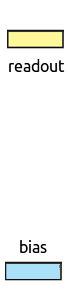
\includegraphics[height=.2\textheight]{LegendConcept.png}
% 		\vspace*{19pt}
% 	\end{subfigure}
% 	\subfig[.43]{3DConcept.png}{.2}{3D}
% 	\caption{Comparison of the planar and the 3D detector concepts}
% 	\label{3d1}
% \end{figure}
% The radiation damage created by the \ac{HL-LHC} will become a big challenge for the innermost tracking detectors. 
After large irradiation, all detector materials become trap limited with a \ac{MFP} below \SI{75}{\micro\meter}. The concept of a 3D detector is a possible way to reduce the drift distance below the this \ac{MFP}. More details about the fabrication and the functionality can be found in \cite{3D}, \cite{parker}.\par
%%%%%%%%%%%%%%%%%%%%%%% CONCEPT %%%%%%%%%%%%%%%%%%%%%%%%%%%
% Its basic principle is shown in figure \vref{3d1}: In a planer detector the readout and bias electrodes are brought onto the front and back side of the sensor with a thickness $\Updelta$. The resulting drift distance L of the charge carriers is of the order of $\Updelta$. In the 3D detector the electrodes are put inside of the detector material so that the \acp{MIP} can travel the same distance $\Updelta$ in the material and therefore create the same amount charge carriers but L is heavily reduced. In case of diamond these electrode columns are drilled with a \SI{800}{\nano\meter} femtosecond laser which converts the diamond into a resistive mixture of carbon phases.\\
%%%%%%%%%%%%%%%%%%%%%%% MULTI %%%%%%%%%%%%%%%%%%%%%%%%%%%%%
In 2015 the first detector was built out of a \pcvd diamond sensor which had 3D readout 
\wrapfigcl{3DMultiResult.png}{.35}{Pulse height of the 3D multi detector}{3d2}
with ganged readout columns as well as a strip metallisation on the same sensor. The thickness of sensor was \SI{\sim500}{\micro\meter} and the 3D cells had a size of \SI{150x150}{\micro\meter}. At this time the column production efficiency was about \SI{92}{\%} \cite{felix}.
% Its square cells are clearly visible and
The mean of the measured pulse height is \SI{13500}{e} which is much higher than \SI{6900}{e} in the strip detector on the same diamond. The strip signal equates to a \ac{CCD} of \SI{192}{\micro\meter} whereas the charge in the 3D would have a \ac{CCD} in a planar detector of \SIrange{350}{375}{\micro\meter} which effectively means that more than \SI{75}{\%} of the created charge was collected for the first time in a \pcvd diamond. The corresponding pulse height distributions are shown in Figure \vref{3d2}. This detector was already a success by showing a working 3D diamond detector. \par
%%%%%%%%%%%%%%%%%%%%%%% FULL 3D %%%%%%%%%%%%%%%%%%%%%%%%%%%
In 2016 a full 3D detector was constructed with dramatic improvements. The number of cells was scaled up from 99 to 1188, the cell size was reduced to to \SI{100x100}{\micro\meter} and the column production efficiency was increased to \SI{99}{\%}. The analysis of this device is still in progress but the first results already show charge in the entire area of the detector and it has the largest charge collection in \pcvd with over \SI{85}{\%} in a contiguous region.\par
%%%%%%%%%%%%%%%%%%%%%%% 3D PIXEL %%%%%%%%%%%%%%%%%%%%%%%%%%
Finally at the end of 2016 the first \pcvd 3D sensor with pixel readout which was metallised and then bump bonded to a CMS pixel \ac{ROC} PSI46digV2.1respin \cite{kornmayer}. The chip was then tuned to a global pixel threshold of \SI{1500}{e}. The preliminary beam test results show an efficiency of \SI{98.5}{\%}. This value is close to the efficiency of a silicon pixel of \SI{99.3}{\%} which was tested in parallel. Compared to the silicon the 3D pixel detector has a relative efficiency of \SI{99.2}{\%}. The loss of \SI{0.8}{\%} is believed to originate from the low field regions between the electrodes.

%============= 6 =============
\section{Conclusion}
By now the technology of diamond detectors is well established in high energy physics. Many of the experiments are already using \acp{BCM} or \acp{BLM} based on \ac{CVD} diamonds. As one of the first pixel projects the ATLAS \ac{DBM} started taking data and was recommissioned for the \SI{13}{\tera\electronvolt} collisions.\\
The diamond material was proven to be very radiation hard and the signal behaviour after the irradiation with various particle species and energies is very well understood for both \sccvd and \pcvd diamonds. In extensive studies it was also found out that \pcvd diamond detectors work reliably and show no signal dependence up to an incident particle flux of \SI{10}{\mega\hertz\per\centi\meter^2}. This could also be shown for irradiated detectors up to fluence of \SI{5e14}{n_{eq}\per \centi\meter^2}.\\
There is also great progress in the development of even more radiation hard devices. The working principle of both 3D strip and pixel detectors could be proven with great success down to cell sizes of \SI{100x100}{\micro\meter}. For the first time more than \SI{80}{\%} of the created charge in the material could be read out. The efficiency of the column drilling process is now above \SI{99}{\%} and the total efficiency of the 3D pixel detectors is very high with \SI{98.5}{\%}.

% ========== ACRONYMS ===========================
\newpage
\section*{List of Acronyms}
\begin{acronym}[Bash]
	\acro{PUC}{pixel unit cell}
	\acro{ROC}{readout chip}
	\acro{TBM}{token bit manager}
	\acro{UB}{ultra black}
	\acro{B}{black}
	\acro{CMS}{Compact Muon Solenoid}
	\acro{LHC}{Large Hadron Collider}
	\acro{HL-LHC}{High Luminosity LHC}
	\acro{CERN}{European Organization for Nuclear Research}
	\acro{DAC}{digital to analogue converter}
	\acro{ADC}{analogue to digital converter}
	\acro{LD}{last DAC}
	\acro{DTB}{digital test board}
	\acro{ATB}{analogue test board}
	\acro{ETH}{Eidgen{\"o}ssische Technische Hochschule}
	\acro{FPGA}{Field Programmable Gate Array}
	\acro{PSI}{Paul Scherrer Institut}
	\acro{HV}{high voltage}
	\acro{TTL}{Transistor-Transistor-Logic}
	\acro{PLL}{phase-locked loop}
	\acro{FIFO}{First In - First Out}
	\acro{HAL}{hardware abstraction layer}
	\acro{API}{application programming interface}
	\acro{GUI}{graphical user interface}
	\acro{CLI}{command line interface}
	\acro{DAQ}{data acquisition}
	\acro{CPU}{central processing unit}
	\acro{PG}{pattern generator}
	\acro{I2C}[I$^{2}$C]{Inter-Integrated Circuit}
	\acro{DUT}{device under test}
	\acro{TCP}{Transmission Control Protocol}
	\acro{TU}{trigger unit}
	\acro{COM}{centre of mass}
	\acro{PSB}{Proton Synchrotron Booster}
	\acro{PS}{Proton Synchrotron}
	\acro{SPS}{Super Proton Synchrotron}
	\acro{ALICE}{A Large Ion Collider Experiment}
	\acro{ATLAS}{A Toroidal LHC Apparatus}
	\acro{LHCb}{Large Hadron Collider beauty}
	\acro{LHCf}{ Large Hadron Collider forward}
	\acro{TOTEM}{TOTal Elastic and diffractive cross section Measurement}
	\acro{SUSY}{supersymmetry}
	\acro{HCAL}{hadronic calorimeter}
	\acro{ECAL}{electromagnetic calorimeter}
	\acro{CTR}{calibrate trigger reset}
	\acro{MIP}{minimum ionising particle}
	\acrodefplural{MIPs}{minimum ionising particles}
	\acro{PM}{photo multiplier}
	\acro{TLU}{trigger logic unit}
	\acro{PH}{pulse height}
	\acro{DC}{double column}
	\acro{DESY}{Deutsches Elektronen-Synchrotron}
	\acro{RAM}{Random-Access Memory}
	\acro{PCB}{printed circuit board}
	\acro{PLT}{Pixel Luminosity Telescope}
	\acro{RPC}{remote procedure calls}
	\acro{CVD}{Chemical Vapour Deposition}
	\acro{sc}{single-crystal}
	\acro{p}{poly-crystalline}
	\acro{BCM}{Beam Condition Monitor}
	\acrodefplural{BCMs}{Beam Condition Monitors}
	\acro{BLM}{Beam Loss Monitor}
	\acrodefplural{BLMs}{Beam Loss Monitors}
	\acro{DBM}{Diamond Beam Monitor}
	\acro{ToF}{time-of-flight}
	\acro{IP}{interaction point}
\end{acronym}

% ========== BIBLIOGRAPHY =======================
\newpage
\bibliographystyle{plain}
\bibliography{refs}

\end{document} 
